\section{Progettazione}
\subsection{Progettazione algoritmo per riconoscimento di elementi in un'immagine frammentata}
Per quanto riguarda il problema della frammentazione dei frames in 4K è stato individuato un apposito algoritmo in grado di effettuare il riconoscimento degli oggetti nei frames presenti in un video senza doverli ridimensionare ma utilizzando la tecnica della frammentazione dell'immagine.
\subsubsection{Scomposizione del frame originale in regioni}
Un frame in 4K viene quindi scomposto in una matrice di R x C sotto-immagini chiamate regioni\gls in modo tale che ogni regione sia efficacemente analizzabile da un modello come Faster R-CNN. Per facilitare l'operazione di riconoscimento degli elementi da parte della rete, ogni regione si sovrappone leggermente con le sue regioni adiacenti. Per definire la quantità di pixels da coinvolgere nella sovrapposizione viene definito uno stride\gls che indica quanti pixels della regione tralasciare, sia in verticale che in orizzontale, prima che cominci quella successiva, ovviamente lo stride deve essere minore della larghezza di una regione.
Una Faster R-CNN dopo aver elaborato singolarmente ogni regione come se fosse una singola immagine darà in output una lista di labels\gls con le seguenti caratteristiche:
\begin{itemize}
\item \textbf{(max-x, max-y)}: coordinate del vertice in alto a sinistra del rettangolo rappresentante la label dell'oggetto riconosciuto; 
\item \textbf{(min-x, min-y)}: coordinate del vertice in basso a destra del rettangolo rappresentante la label dell'oggetto riconosciuto; 
\item \textbf{Categoria\gls}: è un numero naturale che indica la categoria di appartenenza dell'elemento individuato;
\item \textbf{Score\gls}: rappresenta la misura di probabilità che la classificazione ottenuta sia effettivamente quella corretta.
\end{itemize}
Successivamente viene aggiustata la posizione delle labels individuate in modo da traslarle nella loro posizione corretta all'interno dell'immagine originale non frammentata. Questo viene fatto aggiungendo un adeguato offset alle coordinate dei vertici dei box delle labels sulla base della loro regione di appartenenza.
\subsubsection{Rimozione degli elementi individuati più volte all'interno delle aree di sovrapposizione}
A causa della presenza delle aree di sovrapposizione dovute alla struttura delle regioni, gli elementi giacenti in queste particolari zone del frame verranno individuati tante volte quante sono le regioni che si sovrappongono in quella determinata area. Per eliminare le copie duplicate e tenerne solo una viene utilizzato un algoritmo chiamato Average Non-Max Suppression (ANMS) che è una variante del Non-Max Suppression tipicamente utilizzato dai modelli di visione artificiale. Invece che tenere la label con lo score maggiore ed eliminare tutte le altre, come box viene calcolato il box che deriva dalla media dei box di tutte labels e lo score viene calcolato come la media dei loro score.
Questo metodo è fondato sul ragionamento che non bisognerebbe buttare via delle informazioni già possedute ma piuttosto riutilizzarle per scoprire qualcosa di nuovo. Per esempio ad uno stesso elemento visualizzato dentro due sezioni differenti di un' immagine potrebbero venirgli assegnati due score diversi. Mentre NMS conserverebbe solo il valore più alto tra i due, ANMS li utilizzerebbe entrambi per ottenere un valore ancora più affidabile aumentando quindi la veridicità della classificazione.
\subsubsection{Creazione di raggruppamenti di labels correlate} 
A questo punto tutti gli elementi sono stati individuati e classificati ma rimane comunque il problema che, a causa della precedente scomposizione, gli oggetti situati all'interno delle aree di sovrapposizione risulterebbero individuati due o più volte. Come si può vedere in figura 5, questo numero varia in base al numero di regioni sulle quali giace l'oggetto. Il secondo problema è che due elementi \textit{vicini} \footnote{Due label sono considerate vicine se sono intersecate tra di loro ed intersecano lo stesso confine di regione}, anche se classificati nella stessa categoria, non è detto che necessariamente debbano rappresentare lo stesso elemento. Un esempio di questo caso lo si può sempre notare in figura 5. Un caso ancora peggiore lo si ha quando non solo l'elemento è situato su più regioni differenti ma sussiste anche il problema che ogni parte dell'elemento verrebbe classificata in modo diverso a causa della loro ambiguità. Infine, è anche possibile che un oggetto si distribuisca su molte regioni ed ogni sua label presenta dimensioni diverse.
\begin{figure}
\begin{center}
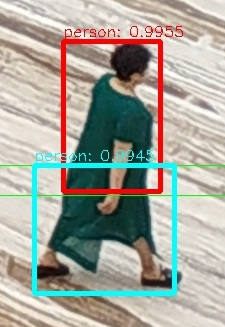
\includegraphics[width=0.2\textwidth, height=0.25\textheight]{images/esempio-frammentazione-1.jpg}
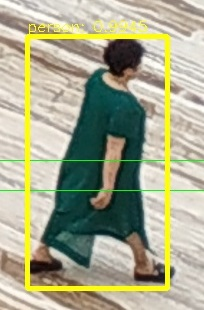
\includegraphics[width=0.2\textwidth, height=0.25\textheight]{images/esempio-frammentazione-4.jpg}
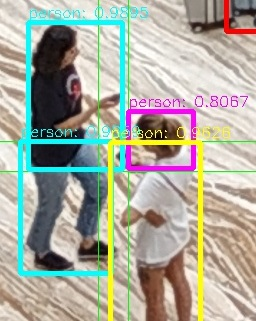
\includegraphics[width=0.2\textwidth, height=0.25\textheight]{images/esempio-frammentazione-2.jpg}
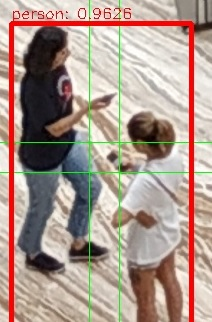
\includegraphics[width=0.2\textwidth, height=0.25\textheight]{images/esempio-frammentazione-3.jpg}
\end{center}
\caption{Esempi di labels erroneamente individuate a causa della frammentazione: nel primo caso la ricostruzione avviene correttamente, nel secondo caso è presente un errore.}
\end{figure}
La soluzione individuata consiste nel raggruppare labels correlate tra loro in insiemi di labels dette raggruppamenti\gls per poi racchiuderli in una label che identifica l'elemento rappresentato dal raggruppamento. Due labels sono in correlazione tra di loro se soddisfano una condizione di correlazione sotto riportata.\\
\textbf{Condizione di correlazione}: Per effettuare un corretto raggruppamento delle labels viene anche tenuta in considerazione la categoria a loro associata tramite la classificazione insieme allo score assegnato. Per definire il risultato della condizione è inoltre necessario stabilire una soglia\gls di probabilità per considerare una label come affidabile o meno. Di seguito vengono riportati i vari casi per decidere se la condizione è vera o falsa.
\begin{itemize}
\item \textbf{True}: Le due labels hanno la stessa categoria ed entrambe con score uguale o maggiore della soglia;
\item \textbf{True}: Le due labels hanno la stessa categoria ma almeno una delle due ha score minore della soglia;
\item \textbf{True}: Le due labels hanno categoria diversa ma almeno una delle due ha score minore della soglia;
\item \textbf{False}: Le due labels hanno categoria diversa ed entrambe con score uguale o maggiore della soglia;
\end{itemize}
Prima di cominciare con il raggruppamento, vengono inizialmente individuate tutte le labels che intersecano i confini di regioni causati dalle aree di sovrapposizione o che non distino più di un fissato numero di pixels, detto overlap\gls, da esse. L'overlap viene definito in quanto anche se nell'immagine reale un oggetto interseca un confine di regione è possibile che a causa di errori di imprecisione del modello, il box della label risulti leggermente distaccato dalla linea che rappresenta il confine. E' quindi possibile ovviare a questo problema aumentando lo spessore del confine di tanti pixels quanti indicati nell'overlap.
Per lo stesso motivo precedente, ai fini di controllare se una label interseca un' altra entità o meno viene anche tenuta in considerazione una tolleranza\gls che indica quanto il box della label può essere distante da quell'entità affinché questa venga comunque considerata come intersecata.
Per creare i raggruppamenti di labels è stato ideato il seguente algoritmo:
\begin{enumerate}
\item Vengono tenute solo le labels che intersecano almeno un confine di regione e sono inizializzate come \textit{non controllate};
\item Viene selezionata una label qualsiasi \textit{non controllata} e la si imposta come \textit{controllata};
\item Per ogni label \textit{controllata} ma non ancora \textit{Raggruppata} controlla se ci sono altre labels \textit{non controllate} che rispettino ognuna delle seguenti condizioni:
  \begin{itemize}
  \item Devono essere \textit{vicine} o distanti entro la tolleranza\gls fissata;
  \item Devono rispettare la \textit{condizione di correlazione};
  \item La loro box non deve intersecare una regione al di fuori delle aree di sovrapposizione che sia già intersecata da una qualsiasi label \textit{controllata}\footnote{Questo perché se due labels sono state individuate come elementi distinti all'interno di una regione allora è probabile che lo siano anche nell'immagine intera in quanto viene supposto che un modello non commetta errori di riconoscimento};
  \item Deve essere rispettata una \textbf{condizione di matching}: La posizione delle loro aree deve essere compatibile entro una certa soglia ovvero che, i lati lungo il quale le due labels vengono unite siano tali che la differenza tra quello maggiore e quello minore sia inferiore ad una certa soglia che può essere sia definita come proporzione rispetto ad uno dei due lati oppure un valore in pixels.
  \end{itemize}  
\item Le labels così trovate diventano a loro volta \textit{controllate};
\item Si ripetono i punti 3 e 4 fino a che non sia più possibile trovare ulteriori labels;
\item Tutte le label \textit{controllate} vengono ora classificate come \textit{raggruppate} e viene assegnato un numero progressivo ad ogni label \textit{raggruppata} in modo da identificarne il gruppo di appartenenza;
\item Si ripetono i punti da 2 a 6 fino a che tutte le labels non vengano raggruppate. L'algoritmo in questo modo termina sempre ed è possibile che un raggruppamento comprenda una sola label.
\end{enumerate}
E' da notare che labels intersecanti ma interamente comprese in una sola regione non sono motivo di interesse in quanto l'algoritmo di Non-Maximum Suppression utilizzato dalla rete in fase di post-processing ci assicura che labels intersecanti individuino elementi diversi.
In seguito bisogna trasformare ogni raggruppamento in una nuova label che racchiuda tutte le labels che lo compongono. Per fare questo vengono esaminate le coordinate di ogni vertice di tutte le labels di un raggruppamento in modo tale da trovare quattro nuovi vertici di un rettangolo che soddisfi i requisiti sopra discussi. Il nuovo box così creato andrà a sostituire le labels del rispettivo raggruppamento e per deciderne la categoria e lo score viene applicata una \textbf{regola di classificazione}: categoria e score assegnati saranno pari alla categoria e allo score posseduti dalla label con score maggiore. \\
A questo punto l'algoritmo può dirsi concluso ed è in grado di riconoscere gli elementi in un'immagine in 4K con un'accuratezza accettabile e buona velocità. Tuttavia in casi particolari come quello mostrato in figura figura 5 l'algoritmo commetterebbe un errore di classificazione in quanto individuerebbe due elementi distinti con una sola label comune.
\subsubsection{miglioramento: Raggruppamenti di labels utilizzati come region proposal}
Un ulteriore miglioramento dell'algoritmo potrebbe essere ottenuto utilizzando le labels ottenute dal procedimento descritto in precedenza come nuove regioni sulle quali applicare nuovamente Faster R-CNN per identificare nuovamente gli elementi contenuti nella regione ma con maggiore precisione in quanto questa volta l'area non verrà affetta da problemi di frammentazione dando quindi la possibilità alla rete di esaminare l'oggetto per intero. La regione viene prima inizializzata rimuovendo la sua label e poi ripopolata con le nuove labels identificate dalla rete.
Il primo problema che salta fuori è che durante questo procedimento la rete identificherà nuovamente anche quegli elementi che casualmente si trovavano dentro la regione coinvolta ma che erano già stati trovati anche in precedenza. Tuttavia questo problema viene tranquillamente risolto applicando un algoritmo di Average Non-Max Suppression, utilizzato già in precedenza, per eliminare oggetti quasi completamente sovrapposti. Il secondo problema riguarda ancora gli oggetti che stanno a cavallo tra la regione interessata e l'immagine originale, questa volta però, avendoli già individuati nella loro interezza durante la prima fase è quindi solamente necessario fondere la nuova label con quella già trovata in precedenza. 
Un caso particolare lo si ha quando la la regione in esame risulti essere così estesa da vanificare i vantaggi ottenuti dalla frammentazione. Per far fronte a questo problema basta ridimensionare l'area coinvolta fino a portarla ad avere dimensioni gestibili da un modello. In questo caso la perdita di risoluzione e quindi di dettagli non comporterebbe un grave problema in quanto gli elementi visibili solo grazie all'alta definizione sono già stati individuati nella fase precedente. Nel caso in cui dovessero venire nuovamente identificati verrebbero gestiti dall'ANMS per ottenerne una migliore approssimazione. Questa funzionalità permette di migliorare l'accuratezza quando si vogliono identificare oggetti che si estendono su due o più regioni o per migliorare il riconoscimento di gruppi di elementi sovrapposti e molto vicini tra loro in prossimità di un confine.
\subsection{Progettazione algoritmo per tracciamento di elementi}
Per affrontare il problema del tracciamento degli elementi, viene utilizzato un algoritmo di tracking supportato da una detection applicata ad ogni frame del video al fine di garantirne una migliore accuratezza. Essendo i video in  qualità 4K, per effettuare la detection viene sempre utilizzato l'algoritmo descritto in sezione \textit{4.1} in modo da non ridurre la qualità dei frames.
\subsubsection{Filtro di Kalman}
Lo scopo di un tracker è quello di predire la posizione di un oggetto in un frame a partire dallo storico delle sue locazioni passate per mezzo di un filtro. I trackers implementati utilizzano un filtro di Kalman in quanto essi si rivelano molto efficaci nell'effettuare predizioni anche in sistemi soggetti a continui cambiamenti come lo è per esempio un video. Il secondo vantaggio è quello di garantire una buona resistenza contro i rumori causati da detections imprecise, le quali, possono per esempio avere luogo in presenza di oggetti parzialmente occultati o deformati a causa del loro spostamento. Infine, questa tipologia di filtri sono anche computazionalmente veloci in quanto, una volta implementati, la loro esecuzione si traduce in semplici moltiplicazioni tra matrici.
L'applicazione del filtro di Kalman consiste in due fasi distinte: predizione ed aggiornamento. La prima fase ha come scopo quello di usare la locazione precedente per predire quella attuale effettuando anche una piccola correzione a causa delle variazioni introdotte da possibili fonti esterne. In seguito sono riportate le formule relative alla fase di predizione:
\[
    x\ped{k} = F\ped{k}x\ped{k-1} + B\ped{k}u\ped{k}
\]
\[
    P\ped{k} = F\ped{k}P\ped{k-1}F\ped{k}\ap{T} + Q\ped{k}
\]
Dove x\ped{k} è la predizione della posizione dell'oggetto \textit{x} nel frame \textit{k}, F\ped{k} è il modello di transizione di stato applicato alla posizione x\ped{k-1}, B\ped{k} è una matrice di controllo alla quale viene applicato il vettore di controllo u\ped{k} e rappresentano le variazioni subite da x\ped{k} causate da un'influenza esterna, in questo caso dal movimento dell'oggetto. P\ped{k} è la predizione della covarianza di x\ped{k} mentre Q\ped{k} è la covarianza del processo che genera rumore.
Nella seconda fase, quella di aggiornamento, viene usata la misurazione corrente, che in questo caso sarà il bounding box dell'oggetto tracciato, per rifinire ulteriormente la sua locazione esatta. In seguito sono riportate le formule relative alla fase di aggiornamento:
\[
    x\ped{k}\ap{'} = x\ped{k} + K(z\ped{k}-H\ped{k}x\ped{k})
\]
\[
    P\ped{k}\ap{'} = P\ped{k} - KH\ped{k}P\ped{k}
\]
\[
	K = P\ped{k}H\ped{k}\ap{T}(H\ped{k}P\ped{k}H\ped{k}\ap{T} + R\ped{k})\ap{-1}
\]
Dove x\ped{k}\ap{'} è la nuova stima della posizione ottenuta dopo aver effettuato l'aggiornamento, K è una matrice detta anche guadagno di Kalman, z\ped{k} è il valore misurato, in questo caso corrisponderà alla label individuata con la detection effettuata sul frame k. H\ped{k} è una matrice che serve per scalare z\ped{k} in modo tale da renderlo compatibile con lo stato dell'oggetto tracciato ed infine R\ped{k} è la covarianza di z\ped{k}.
\subsubsection{Assegnazione detection-tracker}
Il passo successivo è quello di abbinare ognuno dei bounding box stimati dai filtri dei trackers con le bounding boxes individuate da una detection.
Questo risultato viene ottenuto tramite un algoritmo di assegnazione conosciuto anche come algoritmo di Kuhn-Munkres. La metrica utilizzata dall'algoritmo è l'IoU tra i box dei trackers e quelli della detection, tale metrica viene spiegata in dettaglio nella sezione \textit{7.1.3}. L'obiettivo dell'algoritmo è quello di assegnare le detections ai trackers massimizzando la somma dell'IoU delle bounding boxes associate. Questa soluzione di basa sul ragionamento che più due bounding boxes sono sovrapposte, più è probabile che esse traccino lo stesso oggetto. Perchè due bounding boxes possano essere associate il loro IoU deve anche essere maggiore o uguale di una certa soglia, detta soglia di IoU, in quanto tra due boxes poco sovrapposte è comunque probabile che non vi sia alcuna correlazione.
Il primo passo dell'algoritmo consiste nel creare una matrice di dimensioni \textit{n} x \textit{m} dove \textit{n} è il numero di oggetti individuati dalla detection e \textit{m} è il numero di trackers. Ogni cella conterrà il valore dell'IoU tra la box predetta dal tracker \textit{i} ed il box \textit{j} individuato dalla detection, con 0<\textit{i}<m e 0<\textit{i}<n.
Se le colonne sono minori delle righe allora bisogna ruotare la matrice in modo che le colonne siano tante almeno quante sono le righe.
(Immagine)
In seguito vengono ripetuti i seguenti passi:
\begin{enumerate}
\item Per ogni riga, sottrarre il valore minimo della riga a tutti gli elementi della stessa riga. In questo modo, in ogni riga sarà presente almeno una cella con valore pari a 0.
\item Per ogni colonna, sottrarre il valore minimo della colonna a tutti gli elementi della stessa colonna. In questo modo, in ogni colonna sarà presente almeno una cella con valore pari a 0.
\item Tracciare delle linee attraverso tutte le righe e le colonne che contengano almeno un elemento pari a 0 in modo tale da tracciare il minor numero di linee possibile.
\item Se sono state tracciate esattamente k=min(n,m) allora l'algoritmo termina qui, altrimenti si procederà con il passo 5.
\item Trova la cella minore che non sia tracciata da alcuna linea e poi sottrarre quel valore a tutte le righe non tracciate, sommare poi quel valore ad ogni colonna tracciata. Infine tornare al passo 3.
\end{enumerate} 
Al termine dell'algoritmo, vengono selezionati \textit{m} zeri dalle celle della matrice tali che ogni zero appartenga ad una sola riga e ad una sola colonna. Le coordinate di queste celle corrisponderanno agli assegnamenti detection-tracker ottimali da attuare nella matrice originale.
(Immagine)
\subsubsection{Gestione delle detections e dei trackers non assegnati}
\subsubsection{miglioramento: Utilizzo dell'hash dell'immagine come metrica di supporto}